\documentclass{beamer}
 
\usepackage[utf8]{inputenc}
\usepackage{graphicx}
 
%Information to be included in the title page:
\title{Hacking on RISC}
\author{Mohammad Yazdani}
\institute{CS 850}
\date{2018}
 
\begin{document}
 
\frame{\titlepage}
 
\begin{frame}
\frametitle{SPARC: Where to begin?}
The process of booloading a toy kernel on SPARC is partly easy, partly interesting and mostly challenging.
\begin{itemize}
    \item OpenFirmware: Boot sequence is determined by a 512 byte table in the start of memory space.
    \item A position-independent binary has to be loaded into memory.
    \item In the binary, the loader starts with the text section
    \item Our boot.S determines the position of a string we want to print, and the printing function.
    \item Sets string pointer and length as 1st and second arguments and then calls the function.
\end{itemize}
\end{frame}

\begin{frame}
    \frametitle{SPARC: Now: ld}
    Then we need to tell ld to:
    \begin{itemize}
        \item Kickout the headers
        \item Add a.out signature
        \item Size of our text section (comes after header)
    \end{itemize}
\end{frame}

\begin{frame}
    \frametitle{ARM: Where to begin?}
    The process of booloading a toy kernel on ARM is much harder than SPARC, mostly because of QEMU.
    \begin{itemize}
        \item Boot starts at reset, or any machine reset starts at reset. Reset is address 0.
        \item ARM has a very good feature and that is the Interrupt Vector Table that is located at reset.
        \item Interrupt and Exception handling is located in the beginning table and it makes the process of implementing them much easier, specially for embedded systems because of simplicity.
        \item Even though it was harder and took longer to boot ARM, the code looks cleaner and the linking process is more straight forward. This is mostly because of the Interrupt Vector Table.
        \item Implementing system calls in ARM (or rather SWI handlers for SVC calls) was also realtively straight forward with some inline assembly.
    \end{itemize}
\end{frame}

\begin{frame}
    \frametitle{After many hours}
    \framesubtitle{SPARC | ARM}
    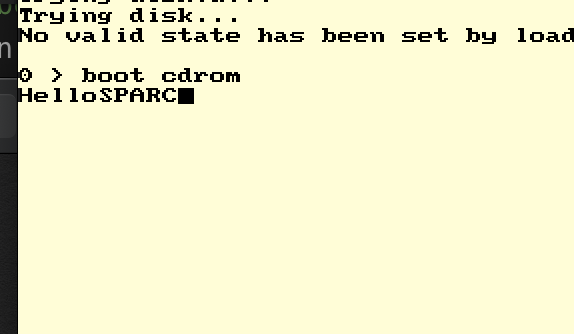
\includegraphics[scale=0.5]{sshot.png}
    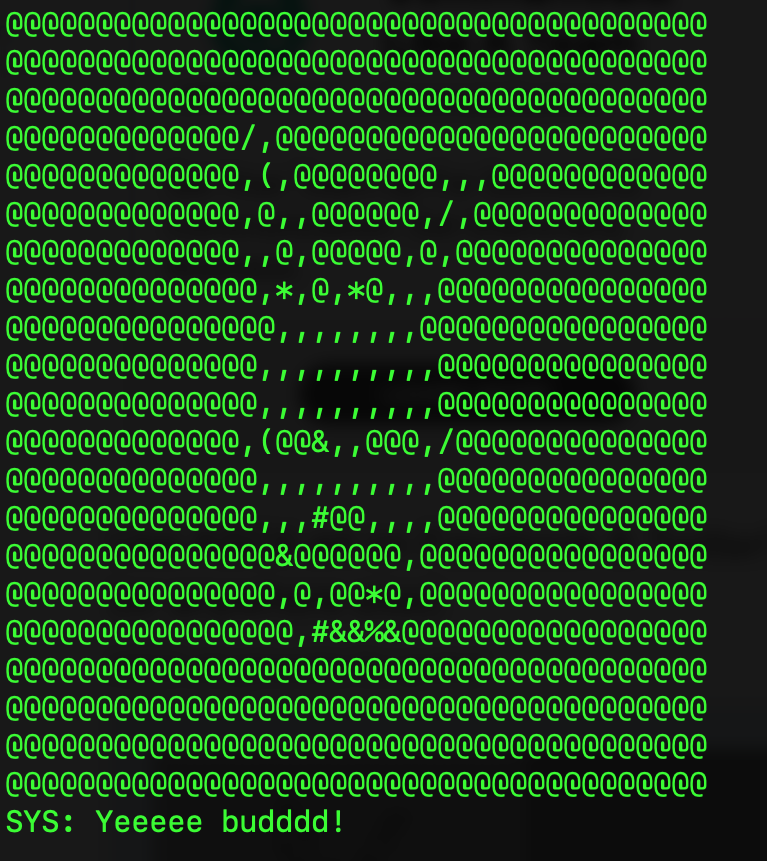
\includegraphics[scale=0.4]{rshot.png}
    
\end{frame}

\begin{frame}
    \frametitle{What I learned and what was interesting:}
    \begin{itemize}
        \item Compilers matter: I faced a lot of problems being able to get the right assembler and the right compiler. In the process of figuring out the bootloader I started to get more and more interested in diving deeper on compilers as an integral part of systems dev.
        \item Compared to what I read on boot loaders for other architectures, the SPARC boot loader is rather more straight forward. The basic process is figuring out your entry point, pointing to something you want to do, return from it and loop.
        \item Even though writing the bootloader did not need as much assembly, you can still see (also after reading some instruction manuals) that ARM is much more complex than SPARC.
    \end{itemize}
\end{frame}

\end{document}
